Our evaluation compares generated conditional samples against theoretical MFTR samples using (i) interpolation cases (conditions inside the training range) and (ii) extrapolation cases (conditions outside the training range). For each case, we use $n=5000$ samples and compute the Kolmogorov--Smirnov statistic (KS), 1D Wasserstein distance, and the MSE/MAE between sorted empirical quantiles.

\subsection{Conditional interpolation vs extrapolation}
Fig.\ \ref{fig:cgan_v16_interp} and Fig.\ \ref{fig:cgan_v16_extra} show three representative examples for interpolation and extrapolation, respectively. Visually, interpolation is consistently better: the QQ points stay closer to the diagonal and the histograms/KDEs follow the theoretical MFTR shape more closely across different condition values. The extrapolation really starts to suffer when $\mu$ goes much farther than 9, the training upper limit, since the distribution then becomes unimodal again with a very long tail, which was unseen during training. We also observe that for $\mu$ very close to 1, the model still tries to produce a bimodal distribution, which is a mismatch with the true unimodal MFTR shape in that case. This suggests that the model has not fully learned the underlying data generation process, but rather has learned to interpolate between the training shapes without fully understanding how the shape changes with $\mu$.

This is also reflected in the metrics in Table\ \ref{tab:cgan_v16_cond_metrics}.The median errors are similar in- vs out-of-range, but the worst-case errors increase out-of-range (e.g., max Wasserstein $\approx 0.109$ vs $\approx 0.050$).

\begin{table}[h]
	\centering
	\caption{Conditional metrics (min / median / max) for interpolation (in-range) and extrapolation (out-of-range).}
	\label{tab:cgan_v16_cond_metrics}
	\small
	\begin{tabular}{lcc}
		\hline
		Metric & In-range (interp.) & Out-of-range (extra.) \\
		\hline
		KS stat. & 0.021 / 0.064 / 0.075 & 0.055 / 0.065 / 0.146 \\
		Wasserstein & 0.016 / 0.045 / 0.050 & 0.025 / 0.045 / 0.109 \\
		MSE & $3.87\times 10^{-4}$ / 0.0024 / 0.0031 & 0.0012 / 0.0026 / 0.014 \\
		MAE & 0.016 / 0.045 / 0.050 & 0.025 / 0.045 / 0.109 \\
		\hline
	\end{tabular}
\end{table}

\begin{figure}[t]
	\centering
	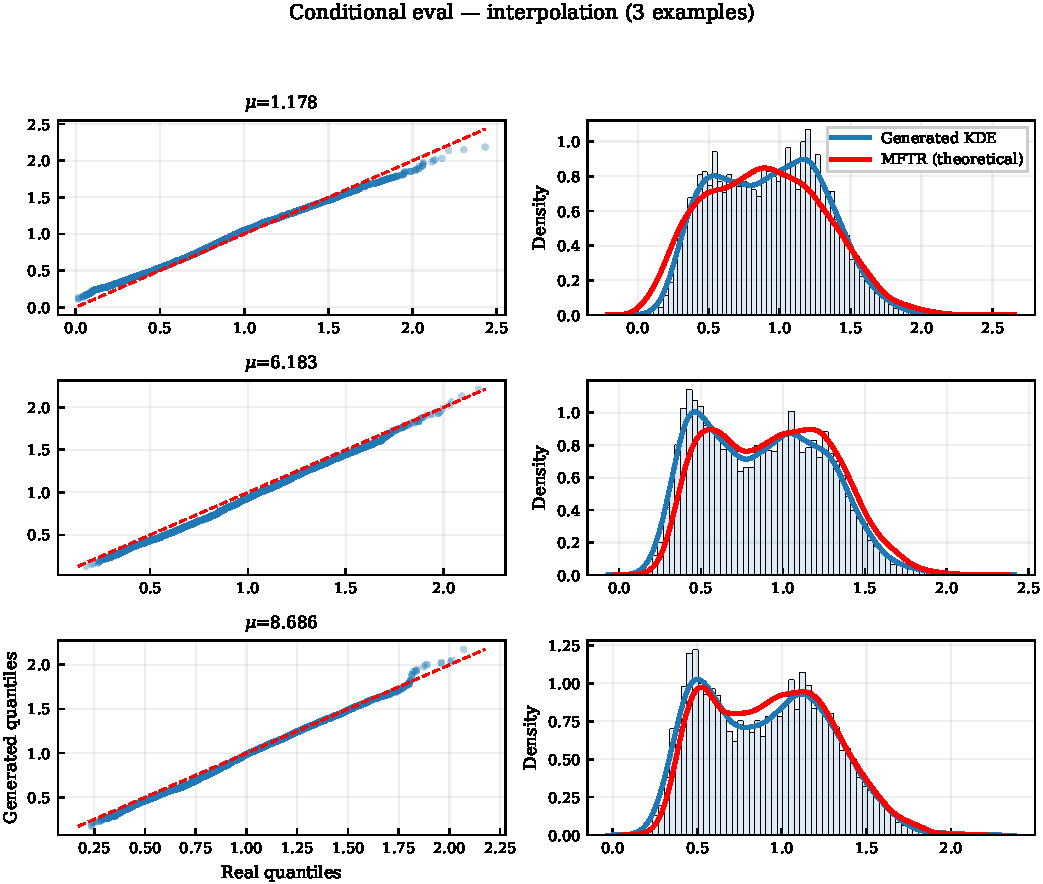
\includegraphics[width=\columnwidth]{../images/cgan_v16_interpolation.pdf}
	\caption{Conditional evaluation (interpolation): three in-range examples.}
	\label{fig:cgan_v16_interp}
\end{figure}

\begin{figure}[t]
	\centering
	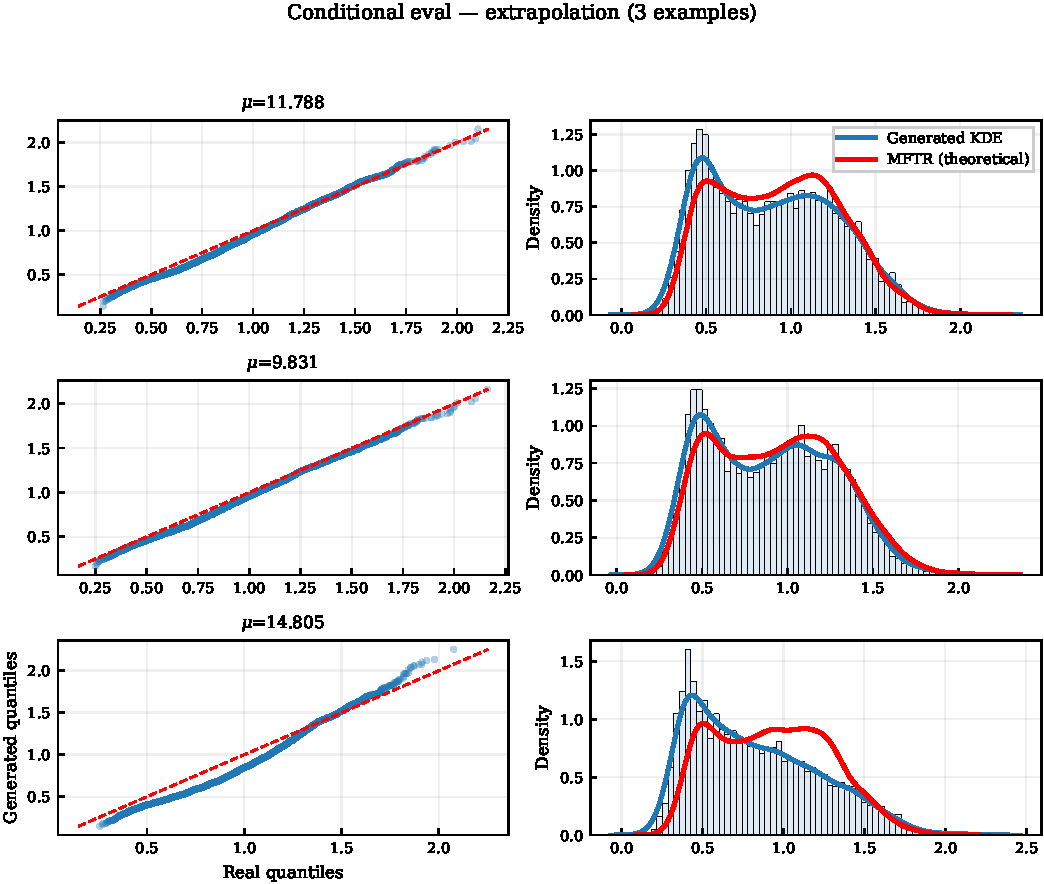
\includegraphics[width=\columnwidth]{../images/cgan_v16_extrapolation.pdf}
	\caption{Conditional evaluation (extrapolation): three out-of-range examples.}
	\label{fig:cgan_v16_extra}
\end{figure}

\subsection{Training dynamics (losses and discriminator probabilities)}
The discriminator and generator losses stabilize very early (Fig.\ \ref{fig:cgan_v16_train_losses}). Across the 150 epochs, the discriminator loss stays close to 1.376 (min 1.373, max 1.377) and the generator loss stays close to 0.80 (min 0.796, max 0.834). Based on these curves, both losses reach a clear plateau by approximately epoch 11.
Even though the losses do not show an obvious downward trend after that point, training for fewer epochs produced noticeably worse conditional fits (verified experimentally). This suggests that in this setting the losses are not a reliable indicator of the final sample quality.

The predicted discriminator probabilities for real and fake samples also remain stable and close to each other (Fig.\ \ref{fig:cgan_v16_train_probs}). On the training set, both probabilities oscillate around 0.45 during most training (means: 0.450 for real and 0.450 for fake). On the validation set, the probabilities are also close to 0.45 on average (means: 0.449 for both), with slightly larger oscillations.

\begin{figure}[t]
	\centering
	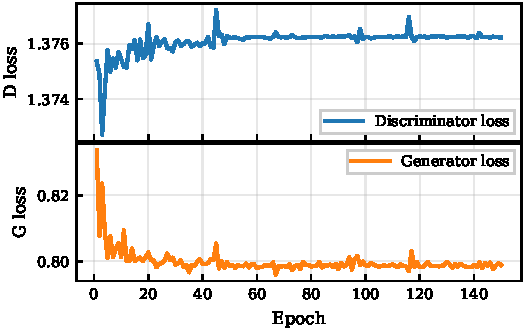
\includegraphics[width=\columnwidth]{../images/cgan_v16_training_losses.pdf}
	\caption{Training curves for generator and discriminator losses.}
	\label{fig:cgan_v16_train_losses}
\end{figure}

\begin{figure}[t]
	\centering
	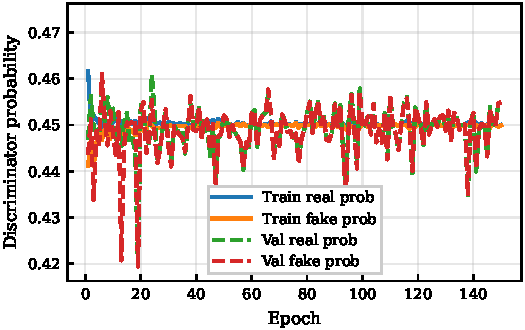
\includegraphics[width=\columnwidth]{../images/cgan_v16_training_probs.pdf}
	\caption{Discriminator predicted probabilities for real and fake samples.}
	\label{fig:cgan_v16_train_probs}
\end{figure}
